\documentclass[12pt]{article}

\usepackage{mhchem}
\usepackage{chemfig}
\usepackage{fancyhdr}
\usepackage{graphicx}
\usepackage[utf8]{inputenc}

\title{Kemi Aflevering 16}
\author{Jeppe Møldrup}
\date{}

\pagestyle{fancy}
\fancyhead[L]{Jeppe Møldrup}
\fancyhead[C]{Kemi 16}
\fancyhead[R]{29/04-2019}

\begin{document}

\maketitle

\section*{Opgave 1}

\begin{enumerate}

        \item[a.] Angiv en egnet indikator til kolorimetrisk titrering
                af syren med natriumhydroxidopløsning

                Jeg har valgt indikatoren Thymolblåt, idet den har et
                farveskift omkring ved pH 8.0, som er aflæst på
                grafen til cirka at være ækvivalenspunktet.

        \item[b.] Bestem syrens molare masse

                Jeg starter med at finde ækvivalenspunktet ved at finde
                ændringen i pH per datapunkt, og så finde hvor denne
                ændring er størst. Jeg har fundet at ændringen er størst
                ved datapunkt 63. Så volumnet er 31.66 mL.\\
                Natriumhydroxiden har en koncentration på 0.0986 M. Så jeg
                ganger med volumnet for at finde stofmængden
                $$0.0986\ M\cdot 31.66\ mL = 0.003127\ mol$$
                Syren og natriumhydroxiden reagerer med et forhold på 1:1.
                Så jeg tager massen af syren og dividerer med stofmængden
                for at finde den molare masse
                $$\frac{0.254\ g}{0.003127\ mol} = 81.87\ g/mol$$
                Så den molare masse af syren er 81.9 g/mol

        \item[c.] Beregn, hvor stor en proceentdel af den ildelugtende syre, der
                findes på baseform i urin med pH 4.5 og temperaturen 25$^{\circ}$C.

                Jeg vil finde $pK_s$, der ligger på grafen ved halvdelen
                af ækvivalenspunktet. Så jeg finder pH for ækvivalenspunktet
                ligesom sidste opgave, som bliver 8.4. Halvdelen af det er
                $$pK_s = \frac{8.68}{2} = 4.2$$
                Nu hvor jeg har $pK_s$ kan jeg finde forholdet mellem den
                ildelugtende syre, og dens korrosponderende base via
                pufferligningen
                $$pH = pK_s+\log \left( \frac{[B]}{[S]} \right)$$
                Så jeg indsætter og finder forholdet
                $$solve(4.5 = 4.2+\log(x),x) \rightarrow x = 1.9953$$
                Så for hver 1 mol syre, er der 1.9953 mol base. Så jeg
                finder hvor mange procent syren udgør
                $$\frac{1\ mol}{1\ mol+1.9953\ mol} = 33.39\%$$
                Så ved pH 4.5 ville 33.4\% være på syreform, dvs. resten
                må være på baseform, så jeg trækker det fra 100\%
                $$100\%-33.4\% = 66.6\%$$
                Så 66.6\% ville være på baseform ved pH 4.5

\end{enumerate}

\section*{Opgave 2}

\begin{enumerate}

        \item[a.] Beregn stofmængden af det euforiserende stof A i denne
                rusdosis

                For at finde stofmængden, dividerer jeg massen med den
                molare masse
                $$n(A) = \frac{m}{M} = \frac{1.10\ g}{149.19\ g/mol} = 0.00737\ mol$$
                Så stofmængden af stoffet A er 0.00737 mol.

        \item[b.] Bestem molekylformlen for A.

                Jeg starter med at tage masseprocenterne for hvert atom
                og se hvor meget af den molare masse de udgør, derefter
                dividerer med atomernes individuelle molare masser for at
                finde hvor mange der er af hver atom.
                $$C:~~~\frac{0.7246\cdot 149.19\ g/mol}{12\ g/mol} \approx 9$$
                $$H:~~~\frac{0.0743\cdot 149.19\ g/mol}{1\ g/mol} \approx 11$$
                $$N:~~~\frac{0.0939\cdot 149.19\ g/mol}{14\ g/mol} \approx 1$$
                $$O:~~~\frac{0.1072\cdot 149.19\ g/mol}{16\ g/mol} \approx 1$$
                Så molekylformlen for stof A er \ce{C9H11NO}

        \item[c.] Argumentor for, hvilke funktionelle grupper der findes
                i X. Generer \ce{^1H-NMR}-spektre af to mulige strukturer for
                A ved 200 MHz.

                Idet der er et O og et N atom, tænker jeg at der må være
                en amid-gruppe i molekylet. Så jeg har lavet de to strukturer\\
                1:\\
                \chemfig{**6(---(-C(=[2]O)-[:-30]N(-[:30]\ce{CH_3})-[-2]\ce{CH3})---)}\\
                2:\\
                \chemfig{**6(---(-C(=[2]O)-[:-30]N(-[:30]\ce{CH2}-[:-30]\ce{CH3})-[-2]H)---)}\\
                Genererede \ce{^1H-NMR}-spektrerne bliver\\
                1:\\
                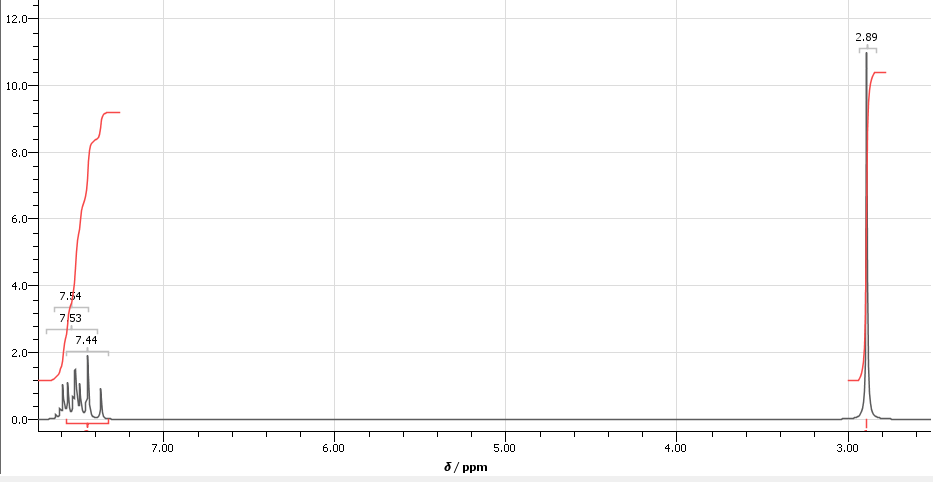
\includegraphics[width=\textwidth]{dia/2c1.png}
                2:\\
                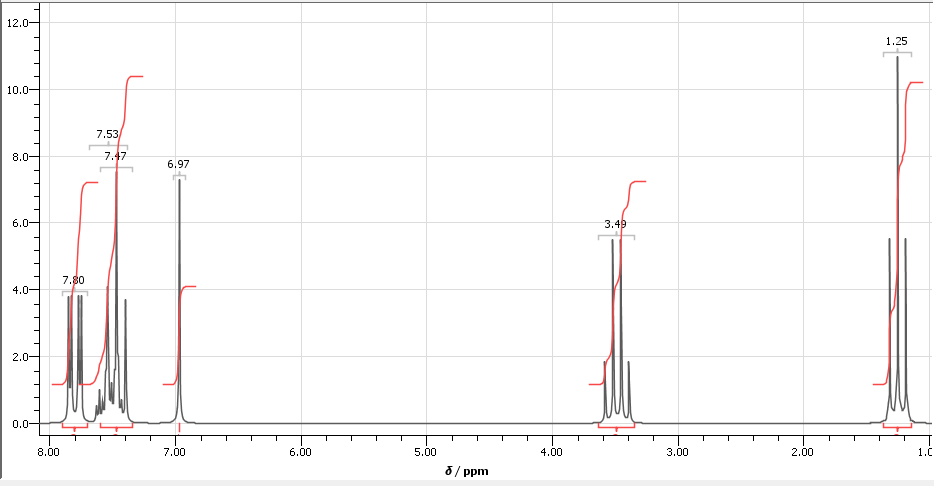
\includegraphics[width=\textwidth]{dia/2c2.png}

        \item[d.] Bestem strukturen for B. Argumenter ud fra integralkurve,
                kemisk skift og koblingsmønstre.



\end{enumerate}

\section*{Opgave 3}

\begin{enumerate}

        \item[a.] Gør rede for, at memantin er en base. Bestem
                $pK_b$ for memantin ved $25^{\circ}$C.

                N-atomet i en amin-gruppe kan optage et ekstra H-atom. Derfor
                kan memantin opføre sig som en base. $pK_s$ for memantin er
                10.7, så jeg kan finde $pK_b$ med formlen
                $$pK_s+pK_b = 14.00 \Leftrightarrow pK_b = 14.00-10.7 = 3.3$$
                Så $pK_b$ for memantin er 3.3

        \item[b.] Angiv reaktionstype for reaktion 1 og for reaktion 3

                Reaktion 1 er en substitutionsreaktion hvor H bliver
                substitueret med Br.

                Reaktion 3 er en opløsning i vand hvor det andet molekyle
                der bliver dannet er ethansyre.

        \item[c.] Gør rede for, hvilke forskelle der er i IR-spektre af
                stofferne B, C og memantin, idet karakteristiske absorptionsbånd
                over 1500 $cm^{-1}$ inddrages.

                C og memantin vil begge give udslag ved omkring 3250-3500
                pga. N-H strækning i aminer. C vil give udslag ved 1600-1750
                pga. C=O stræknignn i carbonyl-forbindelser.

        \item[d.] Forklar grafens forløb. Argumenter ud fra memantins struktur
                og syre-base-egenskaber.

                Memantins opløses let ved lavere pH idet der er flere af den på memantins base form.
                Mens ved højere pH er memantin meget mindre opløselig ved højere pH idet der så vil være flere på syre form.

\end{enumerate}

\section*{Opgave 4}

\begin{enumerate}

        \item[a.] Angiv reaktionstype for reaktionen mellem bromid og bromat.
                
                Reaktionen er en redox-reaktion hvor bromid

        \item[b.] Beregn koncentrationen af det dannede dibrom i reaktionsblandingen i kuvetten, når reaktionen er forløbet til ende

                Der bliver tilsat 20 $\mu$L 0.1 M \ce{KBrO3} som er den begrænsende reaktant. Jeg udregner stofmængden ved at gange
                koncentrationen med volumnet.
                $$0.1\ M\cdot 20\ \mu L = 0.00002\ mol$$
                dibrom bliver dannet af bromat med forholdet 3:1. Så der bliver dannet 0.00006 mol dibrom. Hele volumnet
                er 3000 $\mu$L = 0.003 L. Så koncentrationen af dibromet er
                $$\frac{0.0006\ mol}{0.003\ L} = 0.2\ M$$

        \item[c.] Bestem den molare absorptionskoefficient for dibrom ved 390 nm.

                Jeg bruger lambert beers lov
                $$A = \epsilon \cdot l \cdot c$$
                hvor l = 1 cm, koncentrationen c = 0.2 M og Absorbansen er 0.838. Så jeg indsætter
                $$0.838 = \epsilon \cdot 1\ cm\cdot 0.2\ M = 4.19\ L/(cm\cdot mol)$$
                Så den molare absorptionskoefficient for dibrom ved 390 nm er 4.19 L/(cm mol)

        \item[d.] Vis, at reaktionen er af første orden med hensyn til bromat.
                Angiv en forskrift for koncentrationen af bromat som funktion af tiden.

                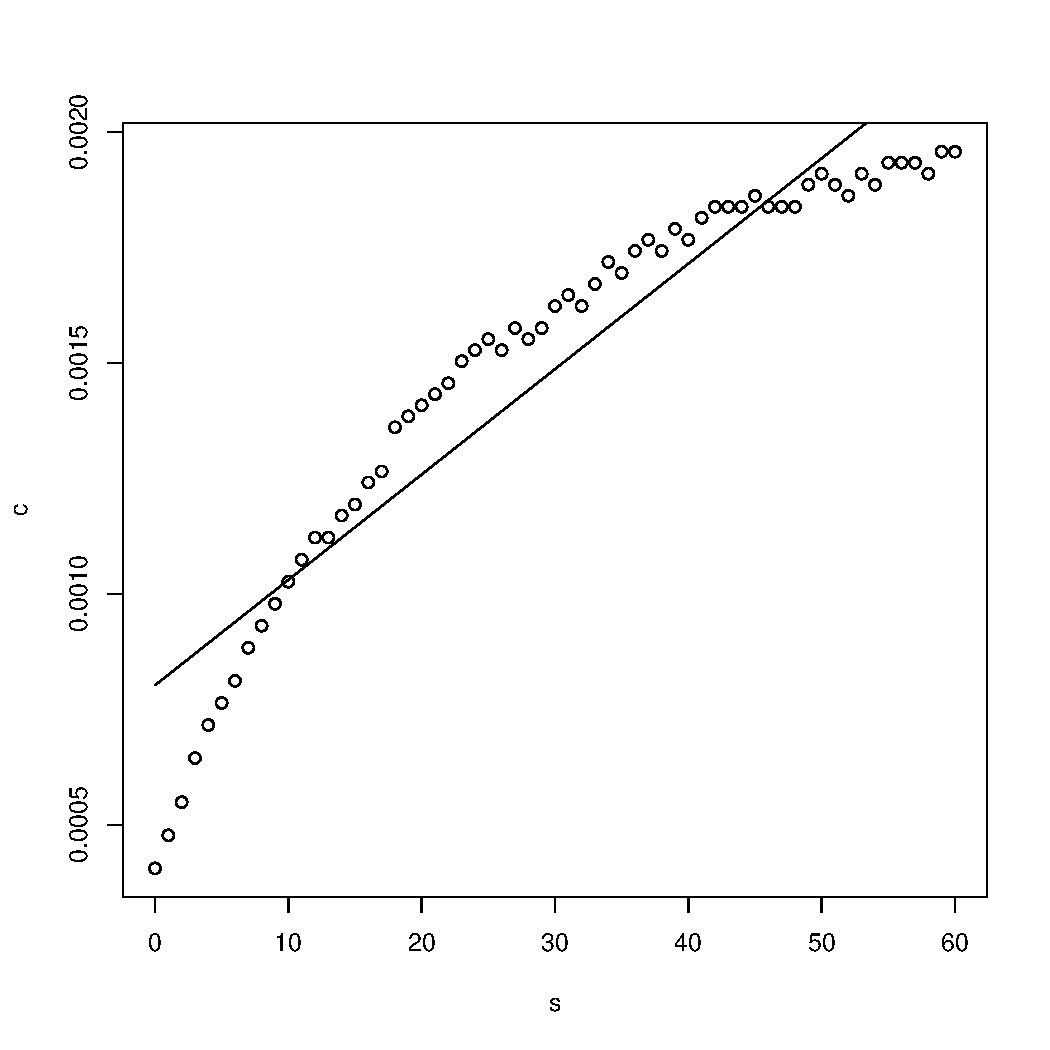
\includegraphics[width=\textwidth]{dia/4d.pdf}
                Den bedste "match" til grafen er den for en første ordens reaktion hvor forskriften for koncentrationen er
                $$[\ce{Br2}] = \frac{A(s)}{\epsilon}$$

        \item[e.] Bestem reaktionsordnerne $y$ og $z$ og reaktionens hastighedskonstant $k$ ved 25$^{\circ}$C.

                I forsøg 1 og 2 er koncentrationen af hydroner konstant. Så derfor afhænger hastigheden kun af
                bromid. Så jeg opstiller de to ligninger
                $$3.7\cdot 10^{-5} = k^*\cdot 0.167^x$$
                $$7.3\cdot 10^{-5} = k^*\cdot 0.333^x$$
                Så kan jeg finde x idet jeg har 2 ligninger med to ubekendte
                $$solve(3.7\cdot 10^{-5} = \frac{7.3\cdot 10^{-5}}{0.333^x}\cdot 0.167^x,x) \rightarrow x = 0.985 \approx 1$$
                ligeledes er koncentrationen af bromid i reaktion 1 og 3 konstant.
                $$3.7\cdot 10^{-5} = k^*\cdot 0.167^x$$
                $$14.6\cdot 10^{-5} = k^*\cdot 0.333^x$$
                så jeg finder x
                $$solve(3.7\cdot 10^{-5} = \frac{14.6\cdot 10^{-5}}{0.333^x}\cdot 0.167^x,x) \rightarrow x = 1.989 \approx 2$$
                Så finder jeg $k$ ved at isolere fra hastighedsudtrykket.
                $$k = \frac{7.3\cdot 10^{-5}}{0.167^2\cdot 0.333^1\cdot (6.7\cdot 10^{-4})^1} = 11.73\ M^{-4}$$
                Så $y = 1$, $z = 2$ og $k = 11.73\ M^{-4}$

\end{enumerate}

\end{document}
